\newpage
\section{Anhang}




\subsection{Tabellen}

\subsubsection{Drehschieberpumpmessungen}

\begin{table}[H]
\tiny
\centering
\begin{tabular}{S [table-format=2.3] S [table-format=2.3] S [table-format=2.3] c }
    \toprule
    \multicolumn{1}{p{3.2cm}}{\centering$\text{Druck Messreihe 1 } $\\$ \text{in }\si{\milli\bar}$} &
    \multicolumn{1}{p{3.2cm}}{\centering$\text{Druck Messreihe 2 } $\\$ \text{in }\si{\milli\bar}$} &
    \multicolumn{1}{p{3.2cm}}{\centering$\text{Druck Messreihe 3 } $\\$ \text{in }\si{\milli\bar}$} &
    \multicolumn{1}{p{3.2cm}}{\centering$\text{Druck gemittelt } $\\$ \text{in }\si{\milli\bar}$} \\
    \midrule
    995.1  & 995.4  & 989.7  & 993.4  \pm 1.5                                 \\
    644    & 640    & 640    & 641.3  \pm 1.1                                 \\
    479    & 439    & 477    & 465    \pm 11                                    \\
    358    & 327    & 357    & 347    \pm 8                                     \\
    265    & 236    & 266    & 256    \pm 8                                     \\
    201    & 177    & 196    & 191    \pm 6                                     \\
    147    & 131    & 144    & 141    \pm 4                                     \\
    103    &  95    & 108    & 102.0  \pm 3.1                                 \\
     75    &  69.8  &  76.9  & 73.9   \pm 1.7                                  \\
     55    &  51    &  56.2  & 54.1   \pm 1.3                                  \\
     40.2  &  36.7  &  41.1  & 39.3   \pm 1.1                                  \\
     29.9  &  26.4  &  30.3  & 28.9   \pm 1.0                                  \\
     21.5  &  19.1  &  21.4  & 20.7   \pm 0.6                                  \\
     15.1  &  14    &  15.5  & 14.9   \pm 0.4                                  \\
     10.8  &  10    &  11.3  & 10.70  \pm 0.31                                \\
      7.9  &   7.3  &   8.5  & 7.90   \pm 0.28                                 \\
      5.9  &   5.5  &   6.1  & 5.83   \pm 0.14                                 \\
      4.5  &   4.2  &   4.6  & 4.43   \pm 0.10                                 \\
      3.5  &   3.2  &   3.6  & 3.43   \pm 0.10                                 \\
      2.8  &   2.6  &   2.9  & 2.77   \pm 0.07                                 \\
      2.2  &   2.1  &   2.3  & 2.20   \pm 0.05                                 \\
      1.9  &   1.6  &   1.9  & 1.80   \pm 0.08                                 \\
      1.6  &   1.5  &   1.6  & 1.567  \pm 0.027                               \\
      1.4  &   1.3  &   1.4  & 1.367  \pm 0.027                               \\
      1.2  &   1.2  &   1.2  & 1.2    \pm 0                                     \\
      1    &   0.99 &   1.1  & 1.030  \pm 0.029                               \\
      0.93 &   0.91 &   0.94 & 0.927  \pm 0.007                               \\
      0.83 &   0.82 &   0.86 & 0.837  \pm 0.010                               \\
      0.76 &   0.74 &   0.77 & 0.757  \pm 0.007                               \\
      0.68 &   0.67 &   0.7  & 0.683  \pm 0.007                               \\
      0.63 &   0.62 &   0.64 & 0.630  \pm 0.005                               \\
      0.59 &   0.57 &   0.6  & 0.587  \pm 0.007                               \\
      0.54 &   0.53 &   0.55 & 0.540  \pm 0.005                               \\
      0.5  &   0.5  &   0.51 & 0.503  \pm 0.0027                             \\
      0.47 &   0.46 &   0.47 & 0.4667 \pm 0.0027                             \\
      0.44 &   0.43 &   0.44 & 0.4367 \pm 0.0027                             \\
      0.41 &   0.41 &   0.42 & 0.4133 \pm 0.0027                             \\
      0.39 &   0.39 &   0.4  & 0.3933 \pm 0.0027                             \\
      0.37 &   0.36 &   0.38 & 0.370  \pm 0.005                               \\
      0.35 &   0.35 &   0.35 & 0.350  \pm 0 \\
      0.33 &   0.33 &   0.33 & 0.33   \pm 0                                    \\
      0.31 &   0.31 &   0.32 & 0.3133 \pm 0.0027                             \\
      0.3  &   0.3  &   0.3  & 0.3    \pm 0                                     \\
      0.28 &   0.28 &   0.29 & 0.2833 \pm 0.0027                             \\
      0.27 &   0.27 &   0.28 & 0.2733 \pm 0.0027                             \\
      0.26 &   0.26 &   0.27 & 0.2633 \pm 0.0027                             \\
      0.25 &   0.25 &   0.25 & 0.25   \pm 0                                    \\
      0.24 &   0.24 &   0.24 & 0.24   \pm 0                                    \\
      0.23 &   0.23 &   0.23 & 0.23   \pm 0                                    \\
      0.21 &   0.22 &   0.23 & 0.220  \pm 0.005                               \\
      0.21 &   0.21 &   0.21 & 0.21   \pm 0                                    \\
      0.2  &   0.2  &   0.21 & 0.2033 \pm 0.0027                             \\
      0.19 &   0.2  &   0.2  & 0.1967 \pm 0.0027                             \\
      0.18 &   0.19 &   0.19 & 0.1867 \pm 0.0027                             \\
      0.17 &   0.18 &   0.18 & 0.1767 \pm 0.0027                             \\
      0.17 &   0.18 &   0.18 & 0.1767 \pm 0.0027                             \\
      0.16 &   0.17 &   0.17 & 0.1667 \pm 0.0027                             \\
      0.16 &   0.16 &   0.16 & 0.16   \pm 0                                    \\
      0.15 &   0.16 &   0.16 & 0.1567 \pm 0.0027                             \\
      0.15 &   0.15 &   0.15 & 0.15   \pm 0                                    \\
      0.14 &   0.15 &   0.15 & 0.1467 \pm 0.0027                             \\
      0.05 &   0.05 &   0.05 & 0.05   \pm  0                        \\
    \bottomrule 
    \end{tabular}
    \caption{Messwerte der Drehschieberpumpenmessreihen für die Druckkurve.}
    \label{tab:dreh_p}
\end{table}



    \begin{table}[H]
        \centering
        \begin{tabular}{S [table-format=2.3] S [table-format=2.3] S [table-format=2.3] c }
            \toprule
            \multicolumn{1}{p{3.2cm}}{\centering$\text{Druck Messreihe 1 } $\\$ \text{in }\si{\milli\bar}$} &
            \multicolumn{1}{p{3.2cm}}{\centering$\text{Druck Messreihe 2 } $\\$ \text{in }\si{\milli\bar}$} &
            \multicolumn{1}{p{3.2cm}}{\centering$\text{Druck Messreihe 3 } $\\$ \text{in }\si{\milli\bar}$} &
            \multicolumn{1}{p{3.2cm}}{\centering$\text{Druck gemittelt } $\\$ \text{in }\si{\milli\bar}$} \\
            \midrule
            0.39 & 0.39 & 0.39 & 0.39  \pm 0 \\
            1.3  & 1.4  & 1.3  & 1.333 \pm 0.027                               \\
            1.4  & 1.5  & 1.4  & 1.433 \pm 0.027                               \\
            1.5  & 1.5  & 1.5  & 1.5   \pm 0                                     \\
            1.6  & 1.6  & 1.6  & 1.6   \pm 0  \\
            1.6  & 1.6  & 1.6  & 1.6   \pm 0  \\
            1.7  & 1.7  & 1.7  & 1.7   \pm 0                                     \\
            1.8  & 1.8  & 1.8  & 1.8   \pm 0                                     \\
            1.9  & 1.9  & 1.9  & 1.9   \pm 0  \\
            1.9  & 1.9  & 1.9  & 1.9   \pm 0   \\
            2    & 2    & 2    & 2.0   \pm 0                                     \\
            2.1  & 2.1  & 2.1  & 2.1   \pm 0                                     \\
            2.1  & 2.2  & 2.1  & 2.133 \pm 0.027                               \\
            2.2  & 2.2  & 2.2  & 2.2   \pm 0                                     \\
            2.3  & 2.3  & 2.2  & 2.267 \pm 0.027                               \\
            2.3  & 2.4  & 2.3  & 2.333 \pm 0.027                               \\
            2.4  & 2.5  & 2.4  & 2.433 \pm 0.027                               \\
            2.5  & 2.5  & 2.5  & 2.5   \pm 0                                     \\
            2.6  & 2.6  & 2.6  & 2.6   \pm 0                                     \\
            2.7  & 2.7  & 2.6  & 2.667 \pm 0.027                               \\
            2.7  & 2.8  & 2.7  & 2.733 \pm 0.027                               \\
            \bottomrule 
            \end{tabular}
            \caption{Messwerte der Leckratenmessung für den Gleichgewichtsdruck $\SI{0.4}{\milli\bar}$ mit der Drehschieberpumpe.}
            \label{tab:dreh_leck_1}
    \end{table}

    \begin{table}[H]
        \centering
        \begin{tabular}{S [table-format=2.3] S [table-format=2.3] S [table-format=2.3] c }
            \toprule
            \multicolumn{1}{p{3.2cm}}{\centering$\text{Druck Messreihe 1 } $\\$ \text{in }\si{\milli\bar}$} &
            \multicolumn{1}{p{3.2cm}}{\centering$\text{Druck Messreihe 2 } $\\$ \text{in }\si{\milli\bar}$} &
            \multicolumn{1}{p{3.2cm}}{\centering$\text{Druck Messreihe 3 } $\\$ \text{in }\si{\milli\bar}$} &
            \multicolumn{1}{p{3.2cm}}{\centering$\text{Druck gemittelt } $\\$ \text{in }\si{\milli\bar}$} \\
            \midrule
            10   & 10   & 10   & 10.0   \pm 0       \\
            19.3 & 19.3 & 19.2 & 19.267 \pm 0.027 \\
            23.1 & 23.1 & 22.9 & 23.03  \pm 0.05   \\
            26.8 & 26.8 & 26.8 & 26.8   \pm 0       \\
            30.3 & 30.3 & 30.4 & 30.333 \pm 0.027 \\
            34.2 & 34.2 & 34.1 & 34.167 \pm 0.027 \\
            38   & 38   & 37.8 & 37.93  \pm 0.05   \\
            41.5 & 41.5 & 41.6 & 41.533 \pm 0.027 \\
            45.5 & 45.5 & 45.3 & 45.43  \pm 0.05   \\
            48.9 & 48.9 & 49.1 & 48.97  \pm 0.05   \\
            53   & 53   & 52.8 & 52.93  \pm 0.05   \\
            56   & 56   & 56.6 & 56.20  \pm 0.16   \\
            60.5 & 60.5 & 60.3 & 60.43  \pm 0.05   \\
            63.8 & 63.8 & 64   & 63.87  \pm 0.05   \\
            67.5 & 67.5 & 68.1 & 67.70  \pm 0.16   \\
            71.5 & 71.5 & 71.1 & 71.37  \pm 0.11   \\
            75   & 75   & 75.2 & 75.07  \pm 0.05   \\
            78.8 & 78.8 & 79.2 & 78.93  \pm 0.11   \\
            82.8 & 82.8 & 82.6 & 82.73  \pm 0.05   \\
            86.8 & 86.6 & 86.2 & 86.53  \pm 0.14   \\
            90.2 & 90.2 & 90.1 & 90.167 \pm 0.027 \\
            \bottomrule 
            \end{tabular}
            \caption{Messwerte der Leckratenmessung für den Gleichgewichtsdruck $\SI{10}{\milli\bar}$ mit der Drehschieberpumpe.}
            \label{tab:dreh_leck_2}
    \end{table}

    \begin{table}[H]
        \centering
        \begin{tabular}{S [table-format=2.3] S [table-format=2.3] S [table-format=2.3] c }
            \toprule
            \multicolumn{1}{p{3.2cm}}{\centering$\text{Druck Messreihe 1 } $\\$ \text{in }\si{\milli\bar}$} &
            \multicolumn{1}{p{3.2cm}}{\centering$\text{Druck Messreihe 2 } $\\$ \text{in }\si{\milli\bar}$} &
            \multicolumn{1}{p{3.2cm}}{\centering$\text{Druck Messreihe 3 } $\\$ \text{in }\si{\milli\bar}$} &
            \multicolumn{1}{p{3.2cm}}{\centering$\text{Druck gemittelt } $\\$ \text{in }\si{\milli\bar}$} \\
            \midrule
            40.1 &  40.2 &  40.1 & 40.133 \pm 0.027 \\
            61.7 &  61.4 &  61.4 & 61.50  \pm 0.08   \\
            75.8 &  75.5 &  75.5 & 75.60  \pm 0.08   \\
            90   &  89.5 &  89.6 & 89.70  \pm 0.12   \\
           104   & 103.7 & 103.7 & 103.80 \pm 0.08  \\
           118.2 & 117.8 & 117.8 & 117.93 \pm 0.11  \\
           133.2 & 131.9 & 131.8 & 132.3  \pm 0.4    \\
           146.4 & 145.9 & 145.9 & 146.07 \pm 0.14  \\
           160.5 & 160.1 & 159.9 & 160.17 \pm 0.14  \\
           174.5 & 174.1 & 174   & 174.20 \pm 0.12  \\
           188.7 & 188.2 & 188.1 & 188.33 \pm 0.15  \\
           202.1 & 201.5 & 201.4 & 201.67 \pm 0.18  \\
           216.1 & 215.6 & 215.5 & 215.73 \pm 0.15  \\
           230.2 & 229.8 & 229.5 & 229.83 \pm 0.17  \\
           244.3 & 245.3 & 243.7 & 244.4  \pm 0.4    \\
           258.6 & 258.2 & 257.8 & 258.20 \pm 0.19  \\
           274.1 & 272.2 & 271.9 & 272.7  \pm 0.6    \\
           286.7 & 285.3 & 285.9 & 285.97 \pm 0.33  \\
           300.8 & 303.2 & 300.1 & 301.4  \pm 0.8    \\
           315   & 314.4 & 314.2 & 314.53 \pm 0.20  \\
           329.1 & 328.5 & 328.3 & 328.63 \pm 0.20  \\
            \bottomrule 
            \end{tabular}
            \caption{Messwerte der Leckratenmessung für den Gleichgewichtsdruck $\SI{40}{\milli\bar}$ mit der Drehschieberpumpe.}
            \label{tab:dreh_leck_3}
    \end{table}

    \begin{table}[H]
        \centering
        \begin{tabular}{S [table-format=2.3] S [table-format=2.3] S [table-format=2.3] c }
            \toprule
            \multicolumn{1}{p{3.2cm}}{\centering$\text{Druck Messreihe 1 } $\\$ \text{in }\si{\milli\bar}$} &
            \multicolumn{1}{p{3.2cm}}{\centering$\text{Druck Messreihe 2 } $\\$ \text{in }\si{\milli\bar}$} &
            \multicolumn{1}{p{3.2cm}}{\centering$\text{Druck Messreihe 3 } $\\$ \text{in }\si{\milli\bar}$} &
            \multicolumn{1}{p{3.2cm}}{\centering$\text{Druck gemittelt } $\\$ \text{in }\si{\milli\bar}$} \\
            \midrule
            80   &  80   &  80   & 80.0    \pm 0      \\
            116.9 & 116   & 115.9 & 116.27 \pm 0.26 \\
            143.9 & 143.1 & 143.1 & 143.37 \pm 0.22 \\
            171   & 170.3 & 170   & 170.43 \pm 0.24 \\
            198   & 197.3 & 196.8 & 197.37 \pm 0.28 \\
            224   & 223.4 & 225.9 & 224.4  \pm 0.6   \\
            251.1 & 252.1 & 253   & 252.1  \pm 0.4   \\
            178.2 & 280   & 280   & 246    \pm 28      \\
            305.2 & 307.1 & 307.2 & 306.5  \pm 0.5   \\
            332.3 & 334.2 & 334.2 & 333.6  \pm 0.5   \\
            359.4 & 361.3 & 361.2 & 360.6  \pm 0.5   \\
            386.2 & 388.1 & 488.1 & 421    \pm 27      \\
            413   & 415.1 & 417.1 & 415.1  \pm 1.0   \\
            439   & 441.3 & 441.7 & 440.7  \pm 0.7   \\
            466.3 & 468.3 & 468.2 & 467.6  \pm 0.5   \\
            492.8 & 494.7 & 494.2 & 493.9  \pm 0.5   \\
            518.8 & 520.7 & 520.8 & 520.1  \pm 0.5   \\
            544.8 & 546.6 & 546.7 & 546.0  \pm 0.5   \\
            570.4 & 572.3 & 572.2 & 571.6  \pm 0.5   \\
            595   & 596.4 & 597.3 & 596.2  \pm 0.5   \\
            620.8 & 620   & 622.5 & 621.1  \pm 0.6   \\
            \bottomrule 
            \end{tabular}
            \caption{Messwerte der Leckratenmessung für den Gleichgewichtsdruck $\SI{80}{\milli\bar}$ mit der Drehschieberpumpe.}
            \label{tab:dreh_leck_4}
    \end{table}



\subsection{Messdaten Turbomolekularpumpe}



\begin{table}[H]
    \small
    \centering
    \begin{tabular}{S [table-format=2.3] S [table-format=2.3] S [table-format=2.3] c }
        \toprule
        \multicolumn{1}{p{3.2cm}}{\centering$\text{Druck Messreihe 1 } $\\$ \text{in }\si{\milli\pascal}$} &
        \multicolumn{1}{p{3.2cm}}{\centering$\text{Druck Messreihe 2 } $\\$ \text{in }\si{\milli\pascal}$} &
        \multicolumn{1}{p{3.2cm}}{\centering$\text{Druck Messreihe 3 } $\\$ \text{in }\si{\milli\pascal}$} &
        \multicolumn{1}{p{3.2cm}}{\centering$\text{Druck gemittelt } $\\$ \text{in }\si{\milli\pascal}$} \\
        \midrule
        166    & 169    & 167    & 167.3 \pm 0.7 \\
        7.8  &   8.73 &  79.8  & 32      \pm 19     \\
        3.3  &   2.98 &   2.7  & 2.99    \pm 0.14 \\
        2.72 &   2.4  &   2.2  & 2.44    \pm 0.12 \\
        2.54 &   2.22 &   2.04 & 2.27    \pm 0.12 \\
        2.42 &   2.13 &   1.95 & 2.17    \pm 0.11 \\
        2.33 &   2.05 &   1.88 & 2.09    \pm 0.11 \\
        2.25 &   1.99 &   1.82 & 2.02    \pm 0.10 \\
        2.2  &   1.94 &   1.78 & 1.97    \pm 0.10 \\
        2.16 &   1.9  &   1.74 & 1.93    \pm 0.10 \\
        2.12 &   1.87 &   1.71 & 1.90    \pm 0.10 \\
        2.09 &   1.84 &   1.68 & 1.87    \pm 0.10 \\
        2.06 &   1.81 &   1.66 & 1.84    \pm 0.10 \\
        2.03 &   1.79 &   1.63 & 1.82    \pm 0.09 \\
        2.01 &   1.77 &   1.62 & 1.80    \pm 0.09 \\
        1.98 &   1.75 &   1.6  & 1.78    \pm 0.09 \\
        1.96 &   1.73 &   1.58 & 1.76    \pm 0.09 \\
        1.94 &   1.71 &   1.57 & 1.74    \pm 0.09 \\
        1.92 &   1.7  &   1.55 & 1.72    \pm 0.09 \\
        1.91 &   1.68 &   1.54 & 1.71    \pm 0.09 \\
        1.9  &   1.67 &   1.53 & 1.70    \pm 0.09 \\
        1    &   1    &   1    & 1.0     \pm 0     \\
        \bottomrule 
        \end{tabular}
        \caption{Messwerte der Turbomolkularpumpenmessreihen für die Druckkurve.\\
        Dabei wurden diese Messwerte direkt an der Pumpe gemessen. }
        \label{tab:turbo_p_pump}
\end{table}


\begin{table}[H]
    \small
    \centering
    \begin{tabular}{S [table-format=2.3] S [table-format=2.3] S [table-format=2.3] c }
        \toprule
        \multicolumn{1}{p{3.2cm}}{\centering$\text{Druck Messreihe 1 } $\\$ \text{in }\si{\milli\pascal}$} &
        \multicolumn{1}{p{3.2cm}}{\centering$\text{Druck Messreihe 2 } $\\$ \text{in }\si{\milli\pascal}$} &
        \multicolumn{1}{p{3.2cm}}{\centering$\text{Druck Messreihe 3 } $\\$ \text{in }\si{\milli\bar}$} &
        \multicolumn{1}{p{3.2cm}}{\centering$\text{Druck gemittelt } $\\$ \text{in }\si{\milli\pascal}$} \\
        \midrule
        496    & 504    & 495    & 498.3 \pm 2.3  \\
        14.2  &  13.2  &  12.8  & 13.40  \pm 0.34 \\
         5.12 &   4.72 &   4.36 & 4.73   \pm 0.18  \\
         4.22 &   3.81 &   3.58 & 3.87   \pm 0.15  \\
         3.96 &   3.61 &   3.4  & 3.66   \pm 0.13  \\
         3.83 &   3.49 &   3.26 & 3.53   \pm 0.14  \\
         3.73 &   3.4  &   3.16 & 3.43   \pm 0.13  \\
         3.66 &   3.33 &   3.09 & 3.36   \pm 0.13  \\
         3.6  &   3.26 &   3.02 & 3.29   \pm 0.14  \\
         3.56 &   3.2  &   2.97 & 3.24   \pm 0.14  \\
         3.52 &   3.16 &   2.93 & 3.20   \pm 0.14  \\
         3.49 &   3.12 &   2.89 & 3.17   \pm 0.14  \\
         3.46 &   3.08 &   2.85 & 3.13   \pm 0.15  \\
         3.44 &   3.05 &   2.82 & 3.10   \pm 0.15  \\
         3.42 &   3.02 &   2.79 & 3.08   \pm 0.15  \\
         3.4  &   3    &   2.76 & 3.05   \pm 0.15  \\
         3.36 &   2.98 &   2.74 & 3.03   \pm 0.15  \\
         3.34 &   2.95 &   2.72 & 3.00   \pm 0.15  \\
         3.31 &   2.93 &   2.7  & 2.98   \pm 0.15  \\
         3.28 &   2.91 &   2.68 & 2.96   \pm 0.14  \\
         3.25 &   2.89 &   2.66 & 2.93   \pm 0.14  \\
         1    &   1    &   1    & 1.0    \pm 0      \\
        \bottomrule 
        \end{tabular}
        \caption{Messwerte der Turbomolkularpumpenmessreihen für die Druckkurve.\\
        Dabei wurden diese Messwerte direkt am Ablassventil gemessen. }
        \label{tab:turbo_p_vent}
\end{table}

\begin{table}[H]
    \small
    \centering
    \begin{tabular}{S [table-format=2.3] S [table-format=2.3] S [table-format=2.3] c }
        \toprule
        \multicolumn{1}{p{3.2cm}}{\centering$\text{Druck Messreihe 1 } $\\$ \text{in }\si{\milli\pascal}$} &
        \multicolumn{1}{p{3.2cm}}{\centering$\text{Druck Messreihe 2 } $\\$ \text{in }\si{\milli\pascal}$} &
        \multicolumn{1}{p{3.2cm}}{\centering$\text{Druck Messreihe 3 } $\\$ \text{in }\si{\milli\bar}$} &
        \multicolumn{1}{p{3.2cm}}{\centering$\text{Druck gemittelt } $\\$ \text{in }\si{\milli\pascal}$} \\
        \midrule
        10.1 &  10.3 &  10   & 10.13 \pm 0.07 \\
        25.1 &  25.8 &  25.2 & 25.37 \pm 0.18 \\
        37.8 &  38.6 &  37.5 & 37.97 \pm 0.27 \\
        49.9 &  50.4 &  49.7 & 50.00 \pm 0.17 \\
        61.5 &  61.8 &  60.3 & 61.2  \pm 0.4   \\
        74.4 &  75.4 &  72.5 & 74.1  \pm 0.7   \\
        91.6 &  92.8 &  88.8 & 91.1  \pm 1.0   \\
       110   & 110   & 107   & 109.0 \pm 0.8  \\
       130   & 131   & 124   & 128.3 \pm 1.8  \\
       147   & 147   & 141   & 145.0 \pm 1.6  \\
       163   & 164   & 157   & 161.3 \pm 1.8  \\
       182   & 183   & 175   & 180.0 \pm 2.1  \\
       202   & 202   & 193   & 199.0 \pm 2.4  \\
        \bottomrule 
        \end{tabular}
        \caption{Messwerte der Leckratenmessung für den Gleichgewichtsdruck $\SI{1e-4}{\milli\bar}$ mit der Drehschieberpumpe. }
        \label{tab:turbo_leck_1}
\end{table}

\begin{table}[H]
    \small
    \centering
    \begin{tabular}{S [table-format=2.3] S [table-format=2.3] S [table-format=2.3] c }
        \toprule
        \multicolumn{1}{p{3.2cm}}{\centering$\text{Druck Messreihe 1 } $\\$ \text{in }\si{\milli\pascal}$} &
        \multicolumn{1}{p{3.2cm}}{\centering$\text{Druck Messreihe 2 } $\\$ \text{in }\si{\milli\pascal}$} &
        \multicolumn{1}{p{3.2cm}}{\centering$\text{Druck Messreihe 3 } $\\$ \text{in }\si{\milli\bar}$} &
        \multicolumn{1}{p{3.2cm}}{\centering$\text{Druck gemittelt } $\\$ \text{in }\si{\milli\pascal}$} \\
        \midrule
        20.2 &  20.4 &  20.3 & 20.30  \pm 0.05    \\
        48.6 &  48.6 &  48.4 & 48.53  \pm 0.05    \\
        80   &  79.6 &  78.2 & 79.3   \pm 0.4      \\
       121   & 122   & 120   & 121.0  \pm 0.5     \\
       162   & 163   & 160   & 161.7  \pm 0.7     \\
       206   & 206   & 205   & 205.67 \pm 0.27   \\
       156   & 160   & 256   & 191    \pm 27        \\
       315   & 318   & 314   & 315.7  \pm 1.0     \\
       376   & 374   & 369   & 373.0  \pm 1.7     \\
       432   &  432 & 428   &   3.0   \pm 1.1 \\
       495   & 494   & 492   & 493.7  \pm 0.7     \\
       563   & 564   & 562   & 563.0  \pm 0.5     \\
       624   & 622   & 620   & 622.0  \pm 0.9     \\
        \bottomrule 
        \end{tabular}
        \caption{Messwerte der Leckratenmessung für den Gleichgewichtsdruck $\SI{2e-4}{\milli\bar}$ mit der Drehschieberpumpe. }
        \label{tab:turbo_leck_2}
\end{table}


\begin{table}[H]
    \small
    \centering
    \begin{tabular}{S [table-format=2.3] S [table-format=2.3] S [table-format=2.3] c }
        \toprule
        \multicolumn{1}{p{3.2cm}}{\centering$\text{Druck Messreihe 1 } $\\$ \text{in }\si{\milli\pascal}$} &
        \multicolumn{1}{p{3.2cm}}{\centering$\text{Druck Messreihe 2 } $\\$ \text{in }\si{\milli\pascal}$} &
        \multicolumn{1}{p{3.2cm}}{\centering$\text{Druck Messreihe 3 } $\\$ \text{in }\si{\milli\bar}$} &
        \multicolumn{1}{p{3.2cm}}{\centering$\text{Druck gemittelt } $\\$ \text{in }\si{\milli\pascal}$} \\
        \midrule
        7   &   7.02 &   6.98 & 7.000  \pm 0.009 \\
        18.4 &  18.3  &  18.2  & 18.30 \pm 0.05  \\
        27.5 &  27.9  &  27.6  & 27.67 \pm 0.10  \\
        36.2 &  37.2  &  36.2  & 36.53 \pm 0.27  \\
        44.6 &  45.3  &  44.6  & 44.83 \pm 0.19  \\
        51.8 &  53.2  &  53    & 52.7  \pm 0.4    \\
        60.1 &  61.6  &  61    & 60.9  \pm 0.4    \\
        67.9 &  69.4  &  68.6  & 68.63 \pm 0.35  \\
        78   &  79.3  &  78.6  & 78.63 \pm 0.31  \\
        89   &  91.4  &  90    & 90.1  \pm 0.6    \\
       101   & 103    & 102    & 102.0 \pm 0.5   \\
       112   & 115    & 113    & 113.3 \pm 0.7   \\
       125   & 128    & 126    & 126.3 \pm 0.7   \\
        \bottomrule 
        \end{tabular}
        \caption{Messwerte der Leckratenmessung für den Gleichgewichtsdruck $\SI{7e-5}{\milli\bar}$ mit der Drehschieberpumpe. }
        \label{tab:turbo_leck_3}
\end{table}


\begin{table}[H]
    \small
    \centering
    \begin{tabular}{S [table-format=2.3] S [table-format=2.3] S [table-format=2.3] c }
        \toprule
        \multicolumn{1}{p{3.2cm}}{\centering$\text{Druck Messreihe 1 } $\\$ \text{in }\si{\milli\pascal}$} &
        \multicolumn{1}{p{3.2cm}}{\centering$\text{Druck Messreihe 2 } $\\$ \text{in }\si{\milli\pascal}$} &
        \multicolumn{1}{p{3.2cm}}{\centering$\text{Druck Messreihe 3 } $\\$ \text{in }\si{\milli\bar}$} &
        \multicolumn{1}{p{3.2cm}}{\centering$\text{Druck gemittelt } $\\$ \text{in }\si{\milli\pascal}$} \\
        \midrule
        5   &  4.99 &  5.04 & 5.010  \pm 0.012 \\
        13.4 & 14.1  & 13.6  & 13.70 \pm 0.17  \\
        21.5 & 22    & 21.4  & 21.63 \pm 0.15  \\
        27.6 & 28.4  & 28.6  & 28.20 \pm 0.25  \\
        33.7 & 35    & 35.2  & 34.6  \pm 0.4    \\
        40.6 & 41.7  & 41.4  & 41.23 \pm 0.27  \\
        46.3 & 47.6  & 47.6  & 47.17 \pm 0.35  \\
        52.4 & 53.6  & 53.7  & 53.23 \pm 0.34  \\
        58.2 & 59.2  & 59.8  & 59.1  \pm 0.4    \\
        64.1 & 65    & 64    & 64.37 \pm 0.26  \\
        70   & 71.6  & 71.9  & 71.2  \pm 0.5    \\
        76.9 & 78.6  & 79.6  & 78.4  \pm 0.6    \\
        84.5 & 87.2  & 87    & 86.2  \pm 0.7    \\
        \bottomrule 
        \end{tabular}
        \caption{Messwerte der Leckratenmessung für den Gleichgewichtsdruck $\SI{5e-5}{\milli\bar}$ mit der Drehschieberpumpe. }
        \label{tab:turbo_leck_4}
\end{table}

\subsection{Aufbau}

\begin{figure}[h]
    \centering
    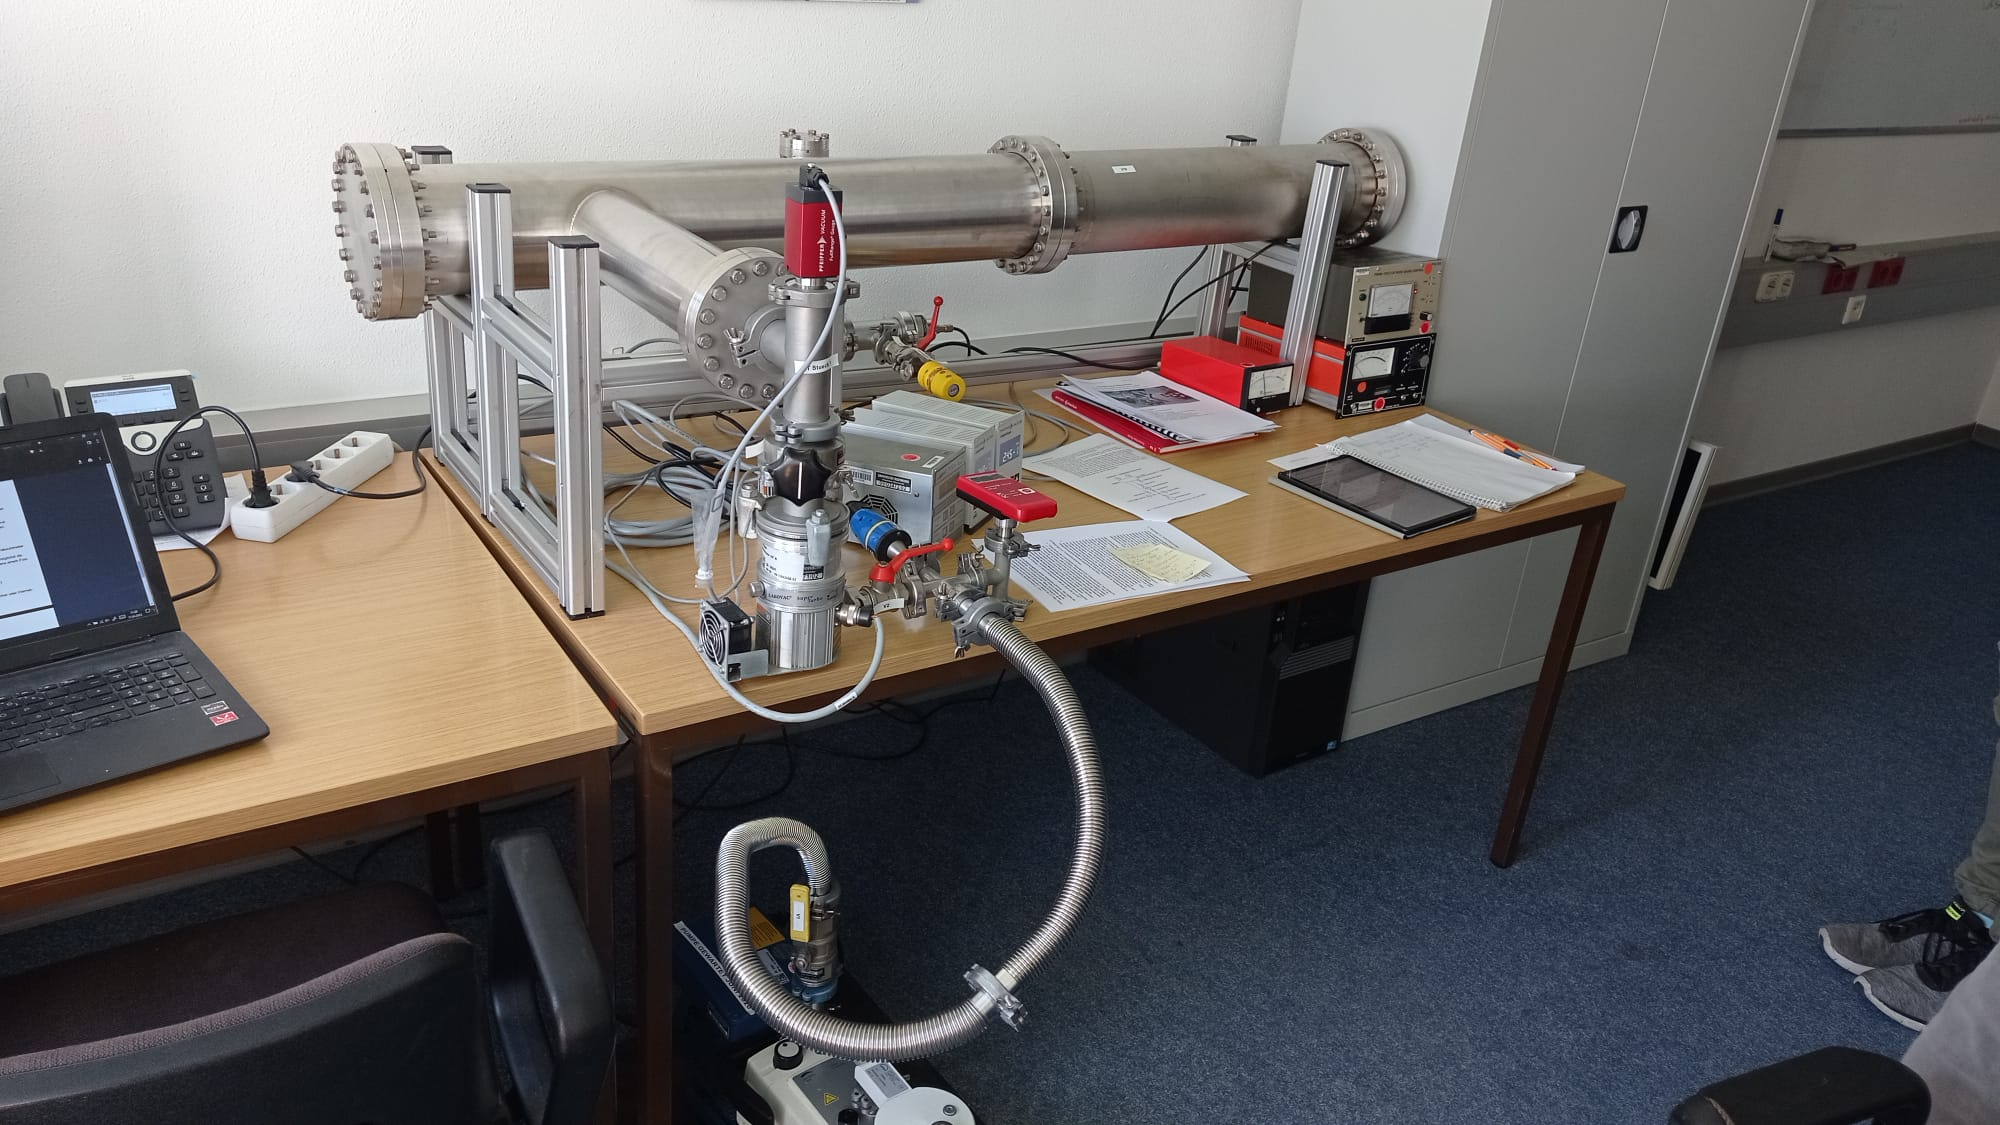
\includegraphics[width=0.7\textwidth]{latex/images/Aufbau.jpeg}
    \caption{Der Versuchsaufbau des Vakuumversuchs}
    \label{img:aufbaufoto}
\end{figure}

\subsection{Messwertfotos}

\begin{figure}[h]
    \centering
    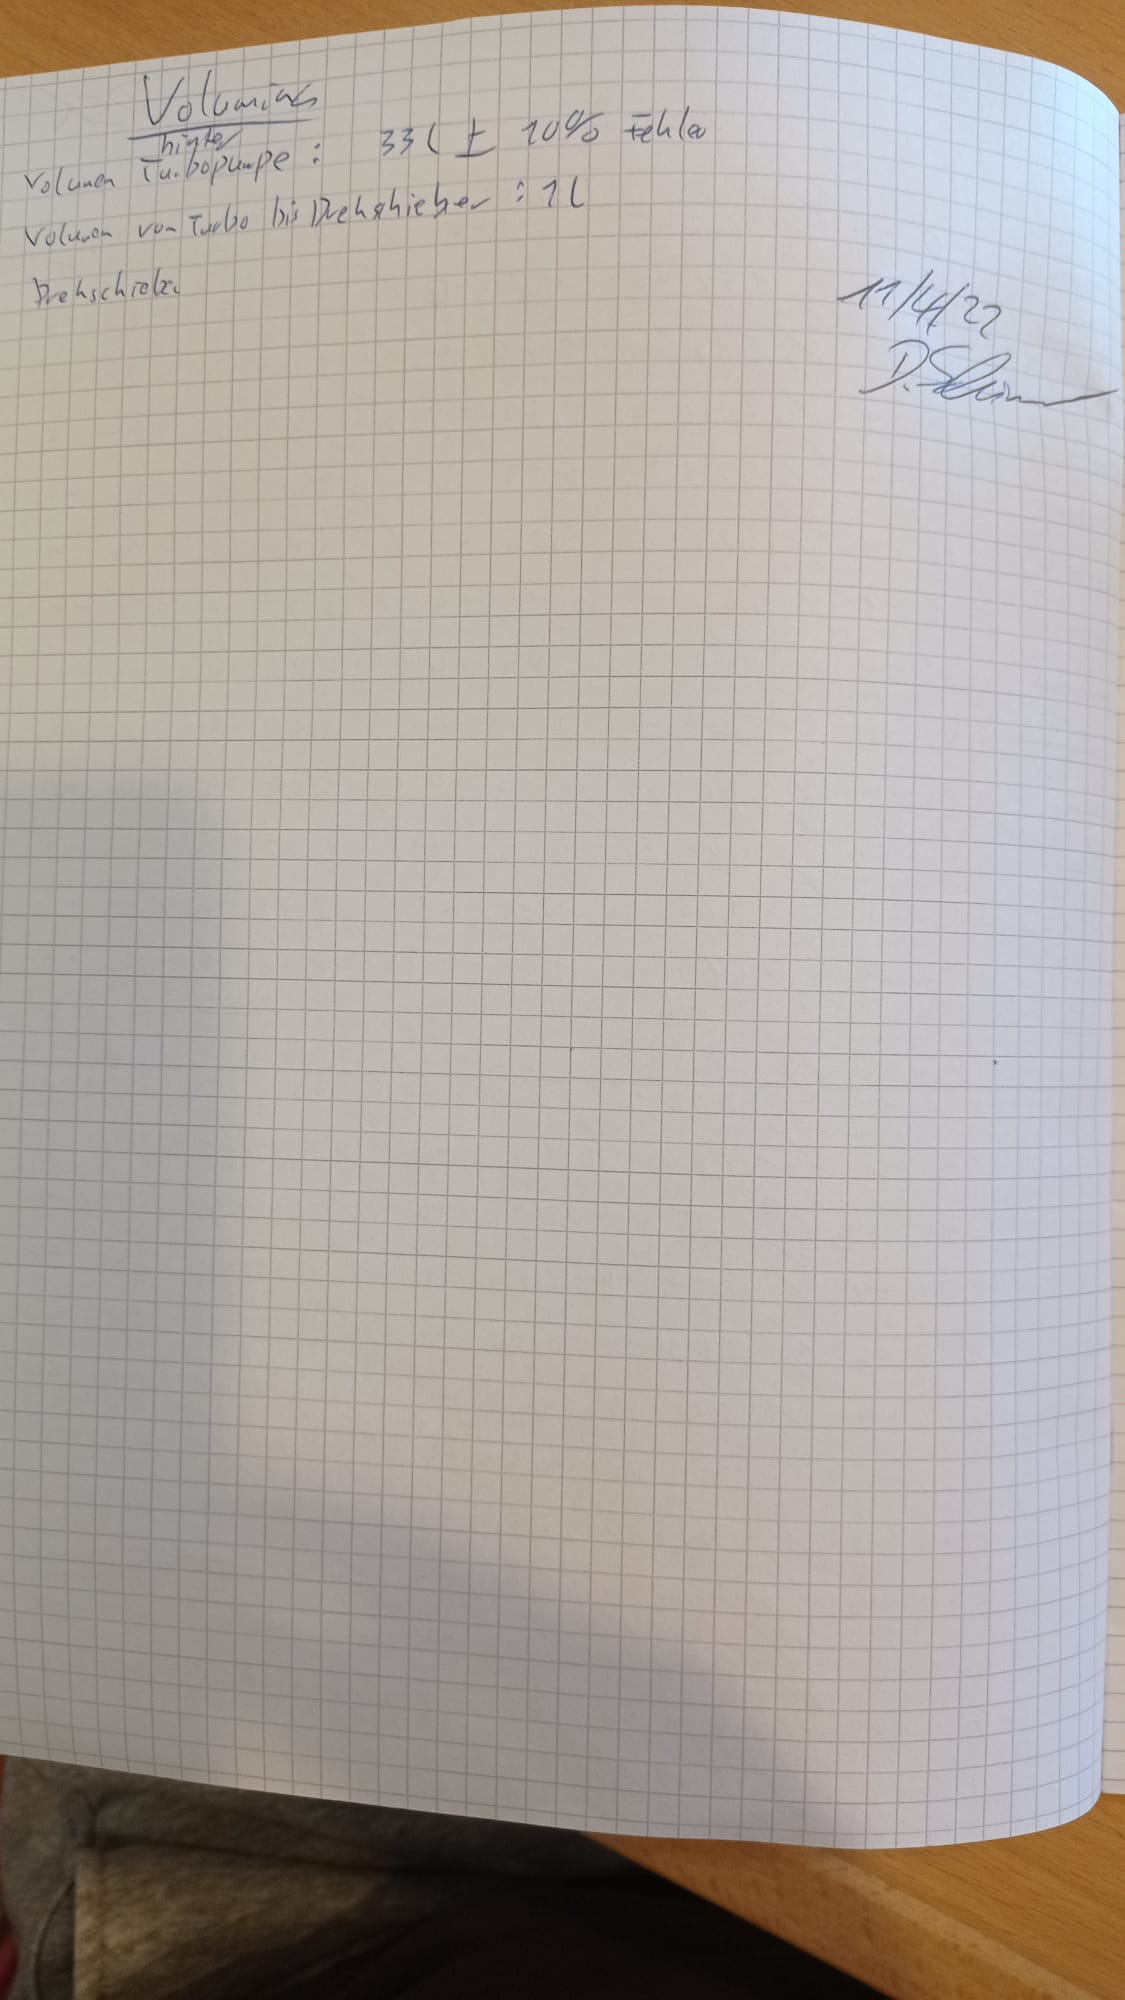
\includegraphics[width=0.7\textwidth]{latex/images/Messwerte_1.jpeg}
    \caption{Die Messwerte des Vakuumversuchs}
\end{figure}

\begin{figure}[h]
    \centering
    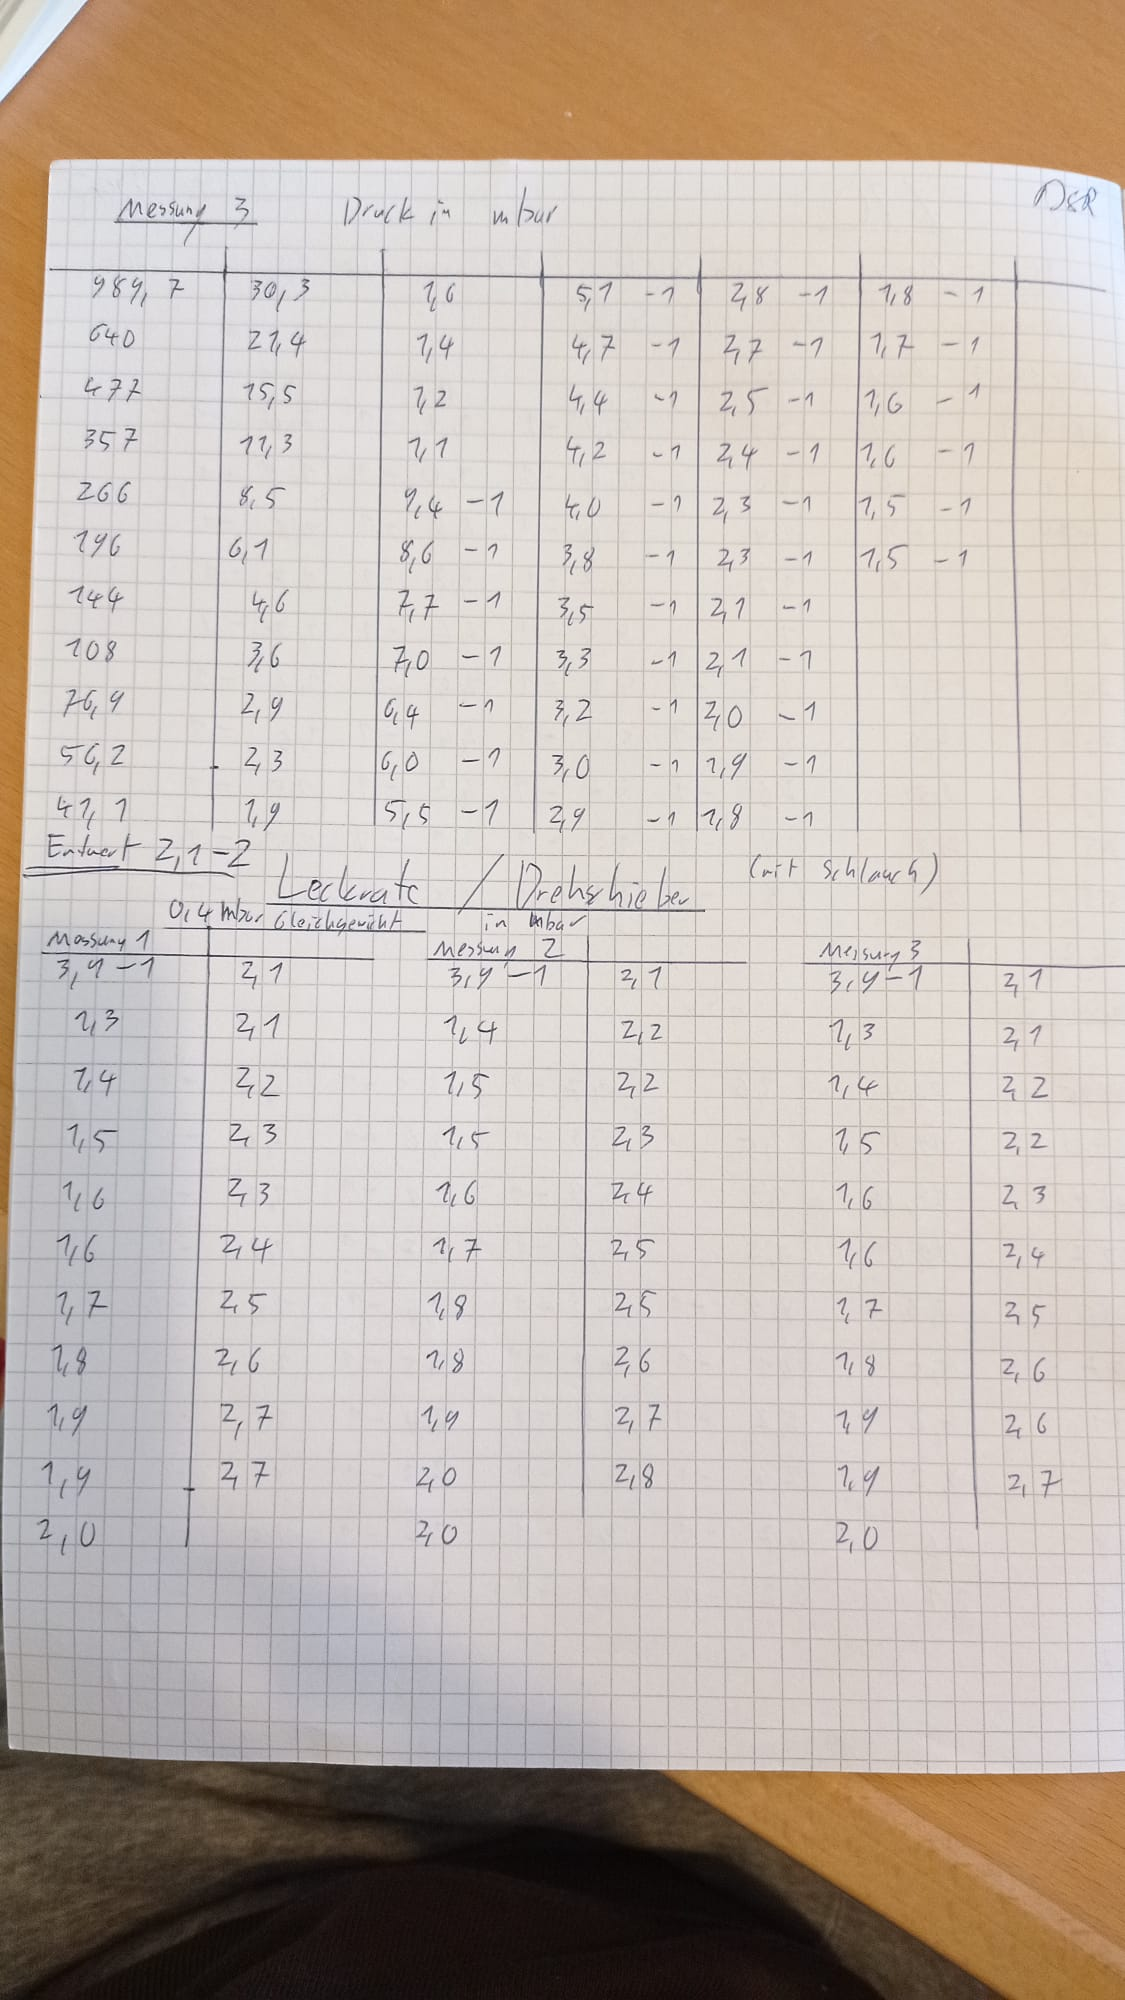
\includegraphics[width=0.7\textwidth]{latex/images/Messwerte_2.jpeg}
    \caption{Die Messwerte des Vakuumversuchs}
\end{figure}

\begin{figure}[h]
    \centering
    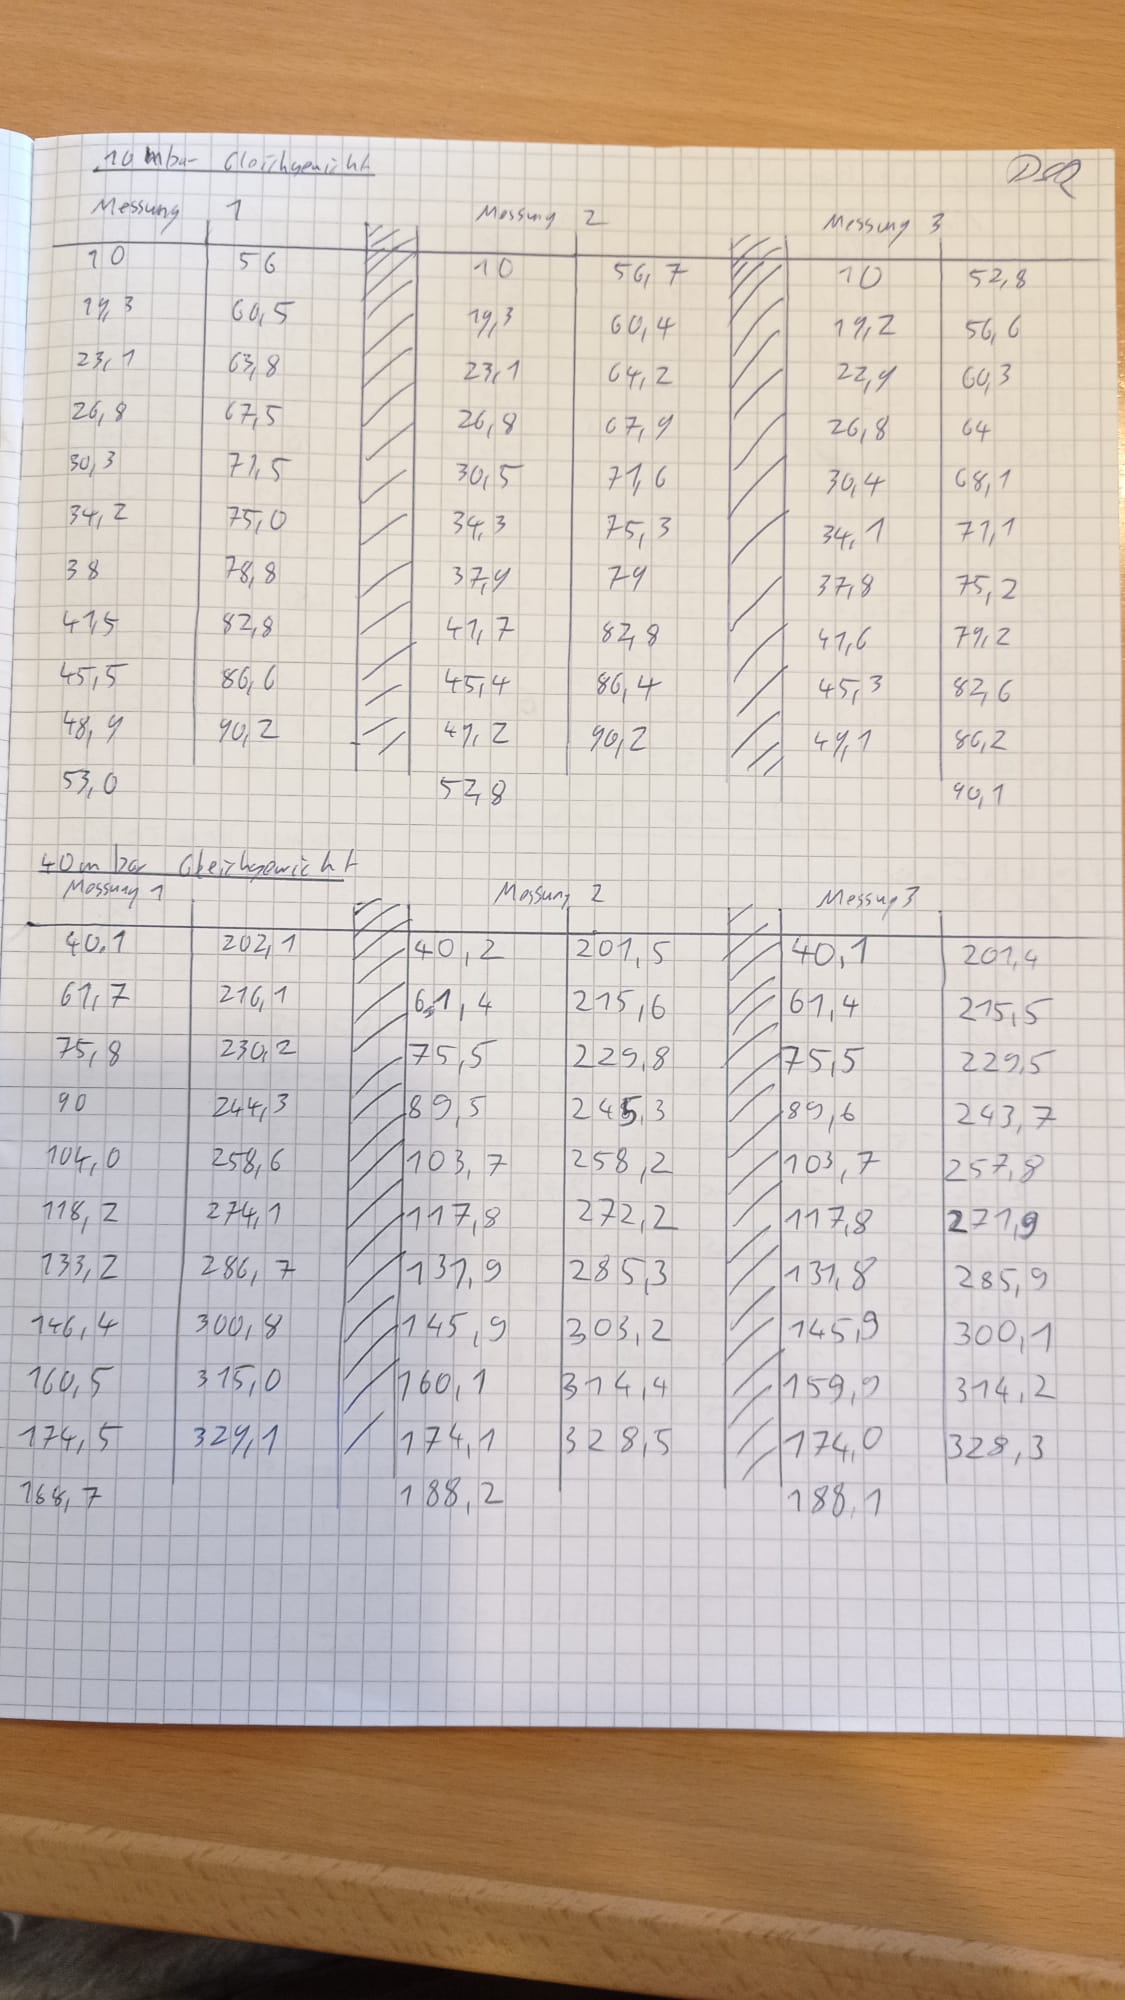
\includegraphics[width=0.7\textwidth]{latex/images/Messwerte_3.jpeg}
    \caption{Die Messwerte des Vakuumversuchs}
\end{figure}


\begin{figure}[h]
    \centering
    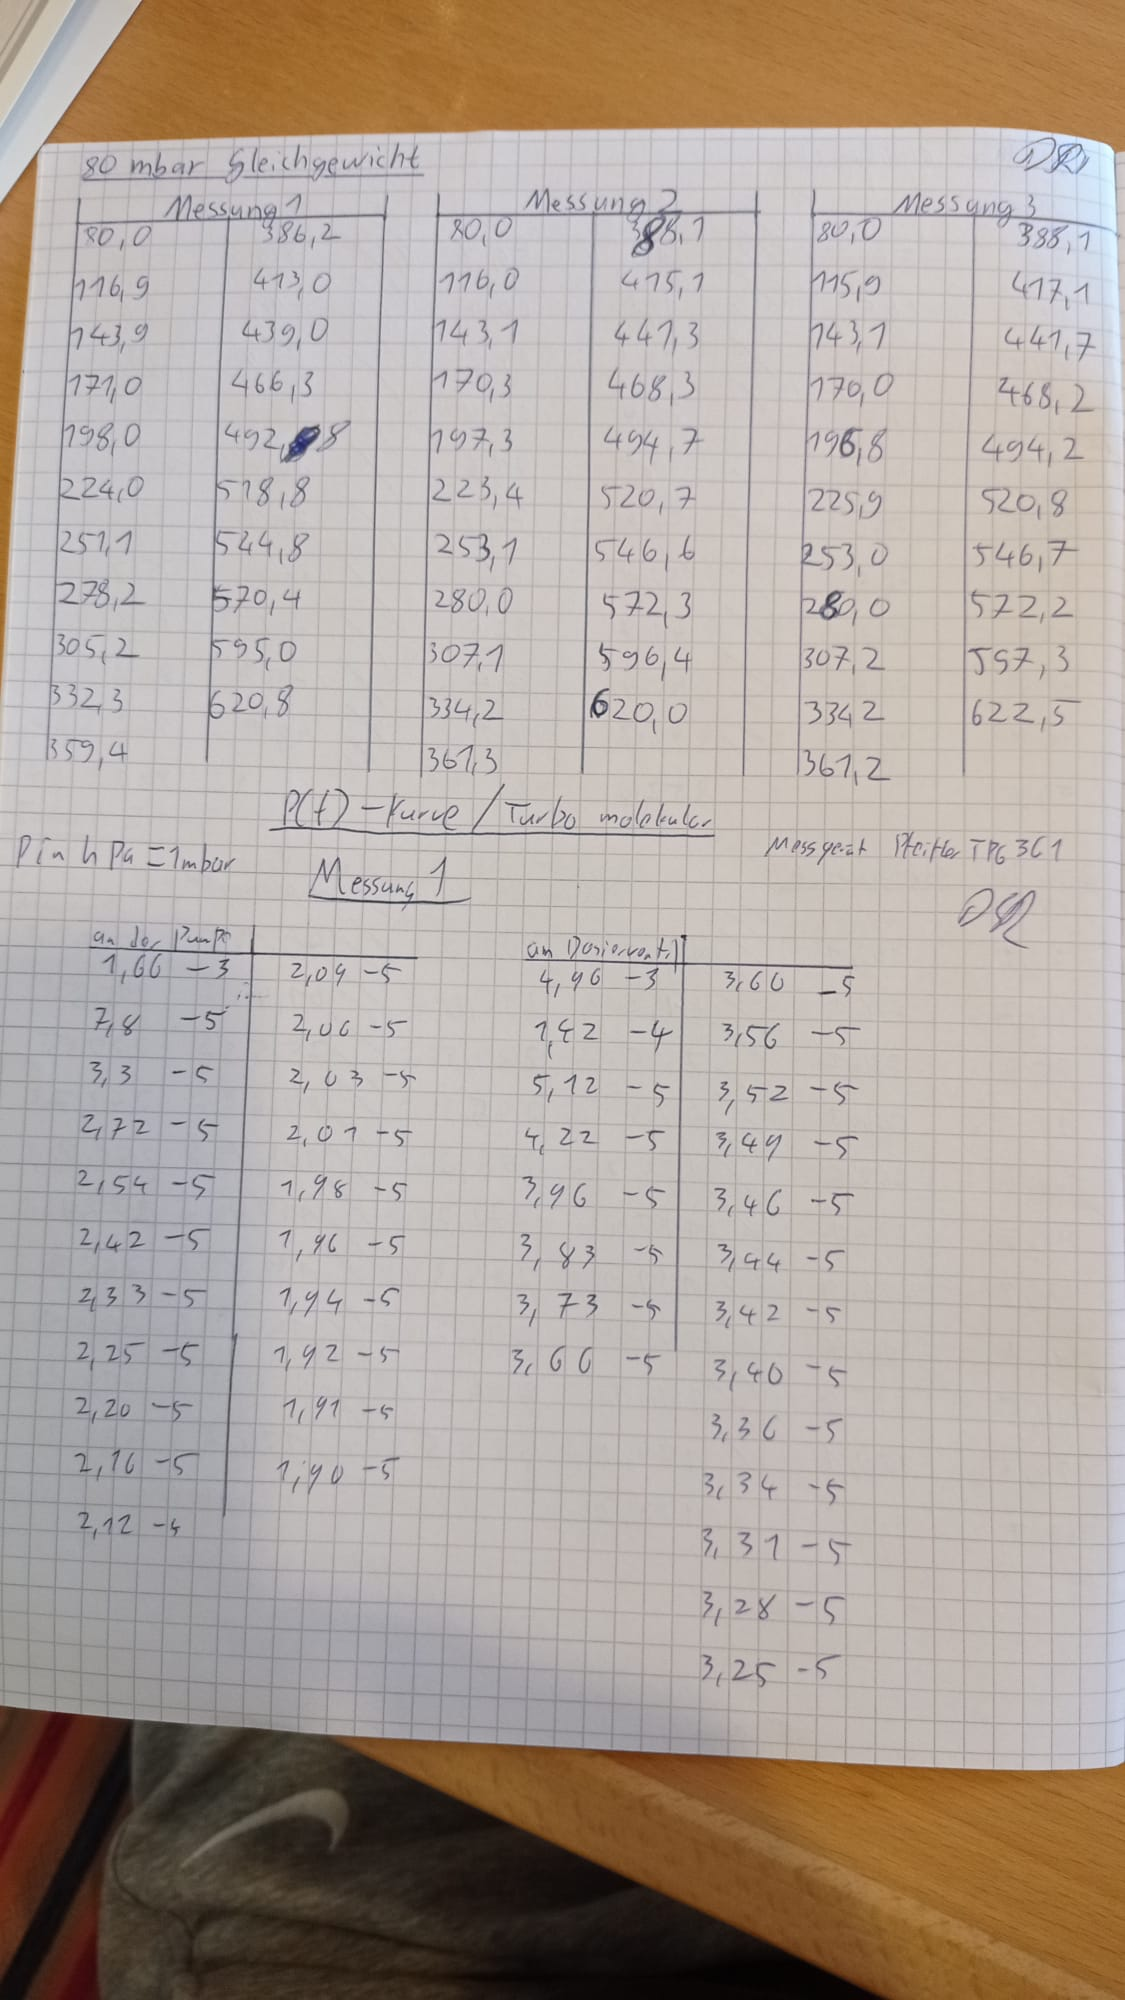
\includegraphics[width=0.7\textwidth]{latex/images/Messwerte_4.jpeg}
    \caption{Die Messwerte des Vakuumversuchs}
\end{figure}


\begin{figure}[h]
    \centering
    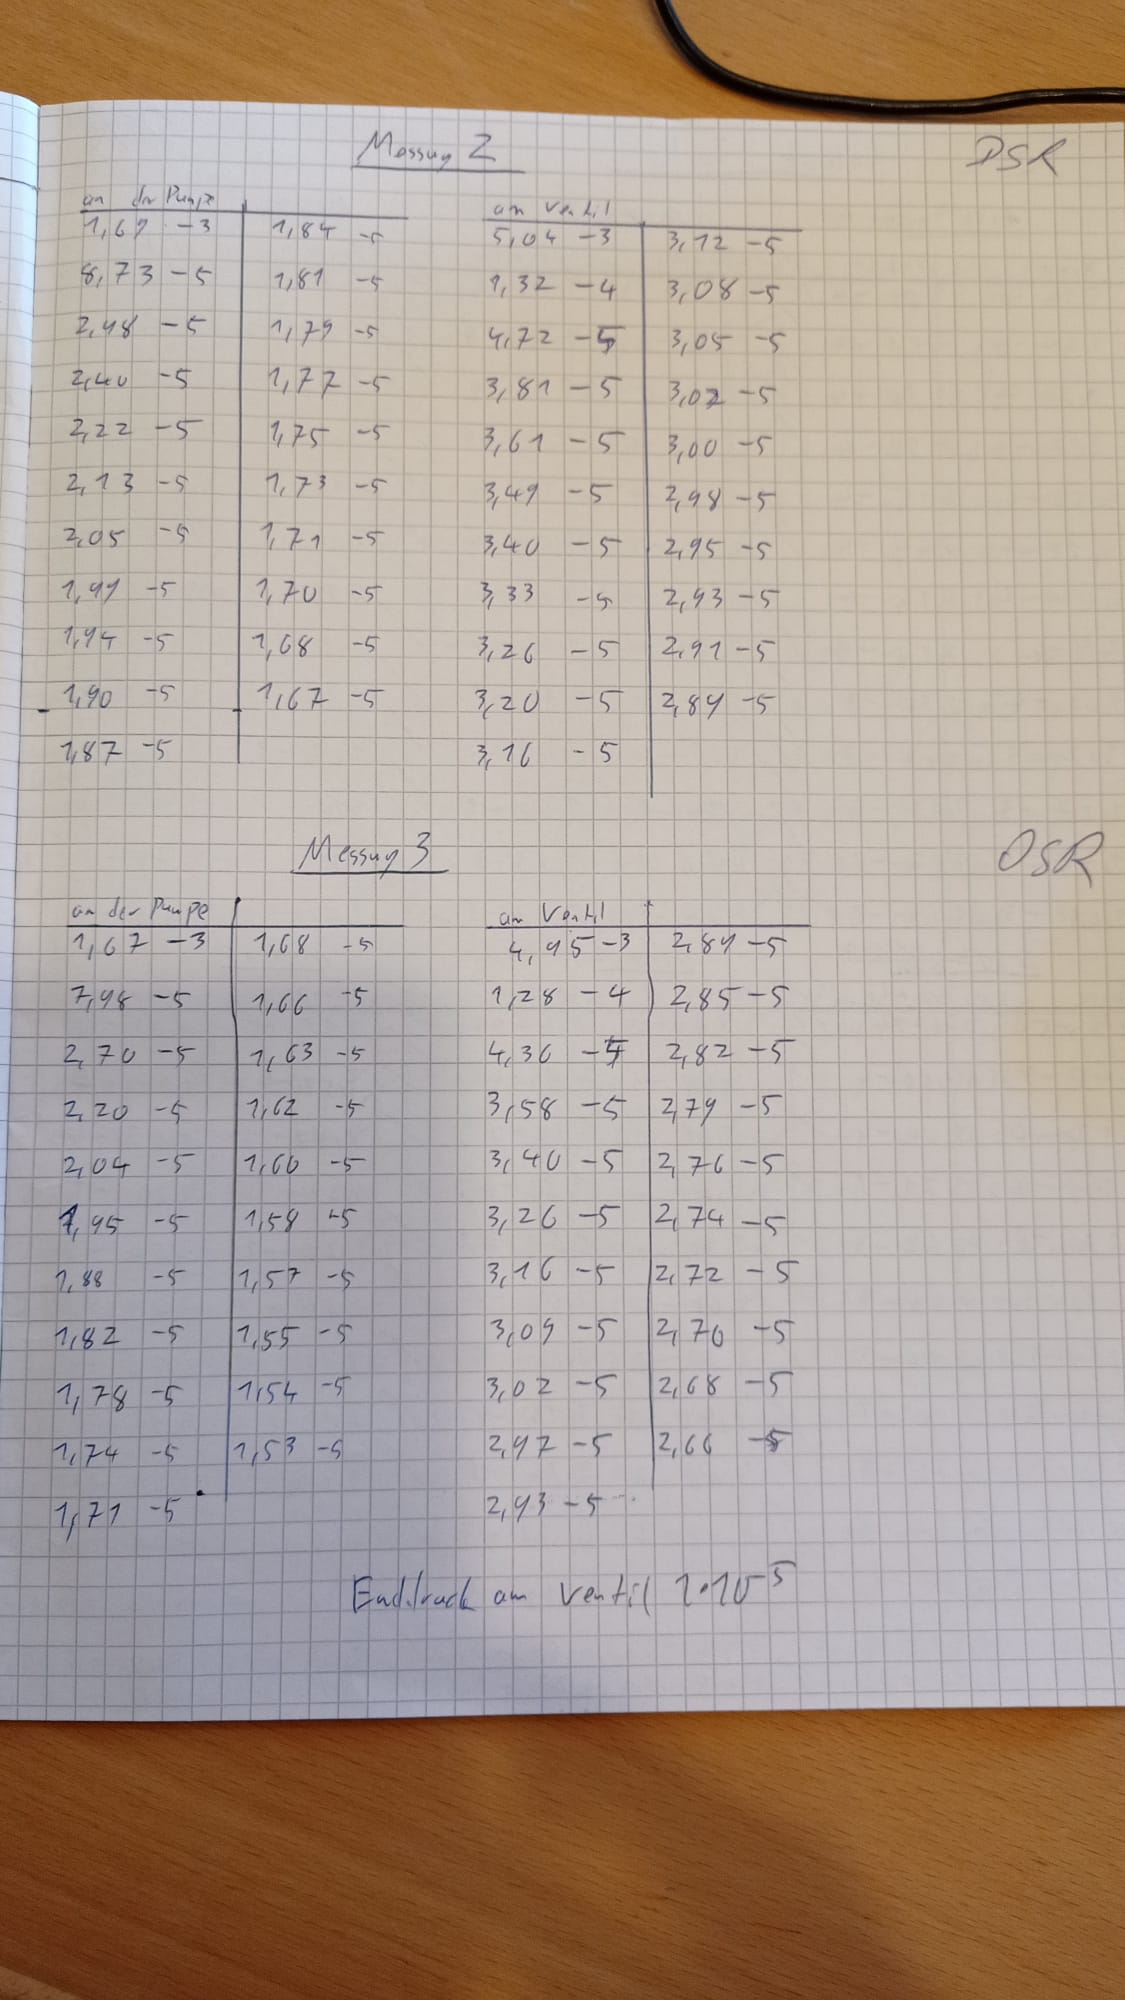
\includegraphics[width=0.7\textwidth]{latex/images/Messwerte_5.jpeg}
    \caption{Die Messwerte des Vakuumversuchs}
\end{figure}

\begin{figure}[h]
    \centering
    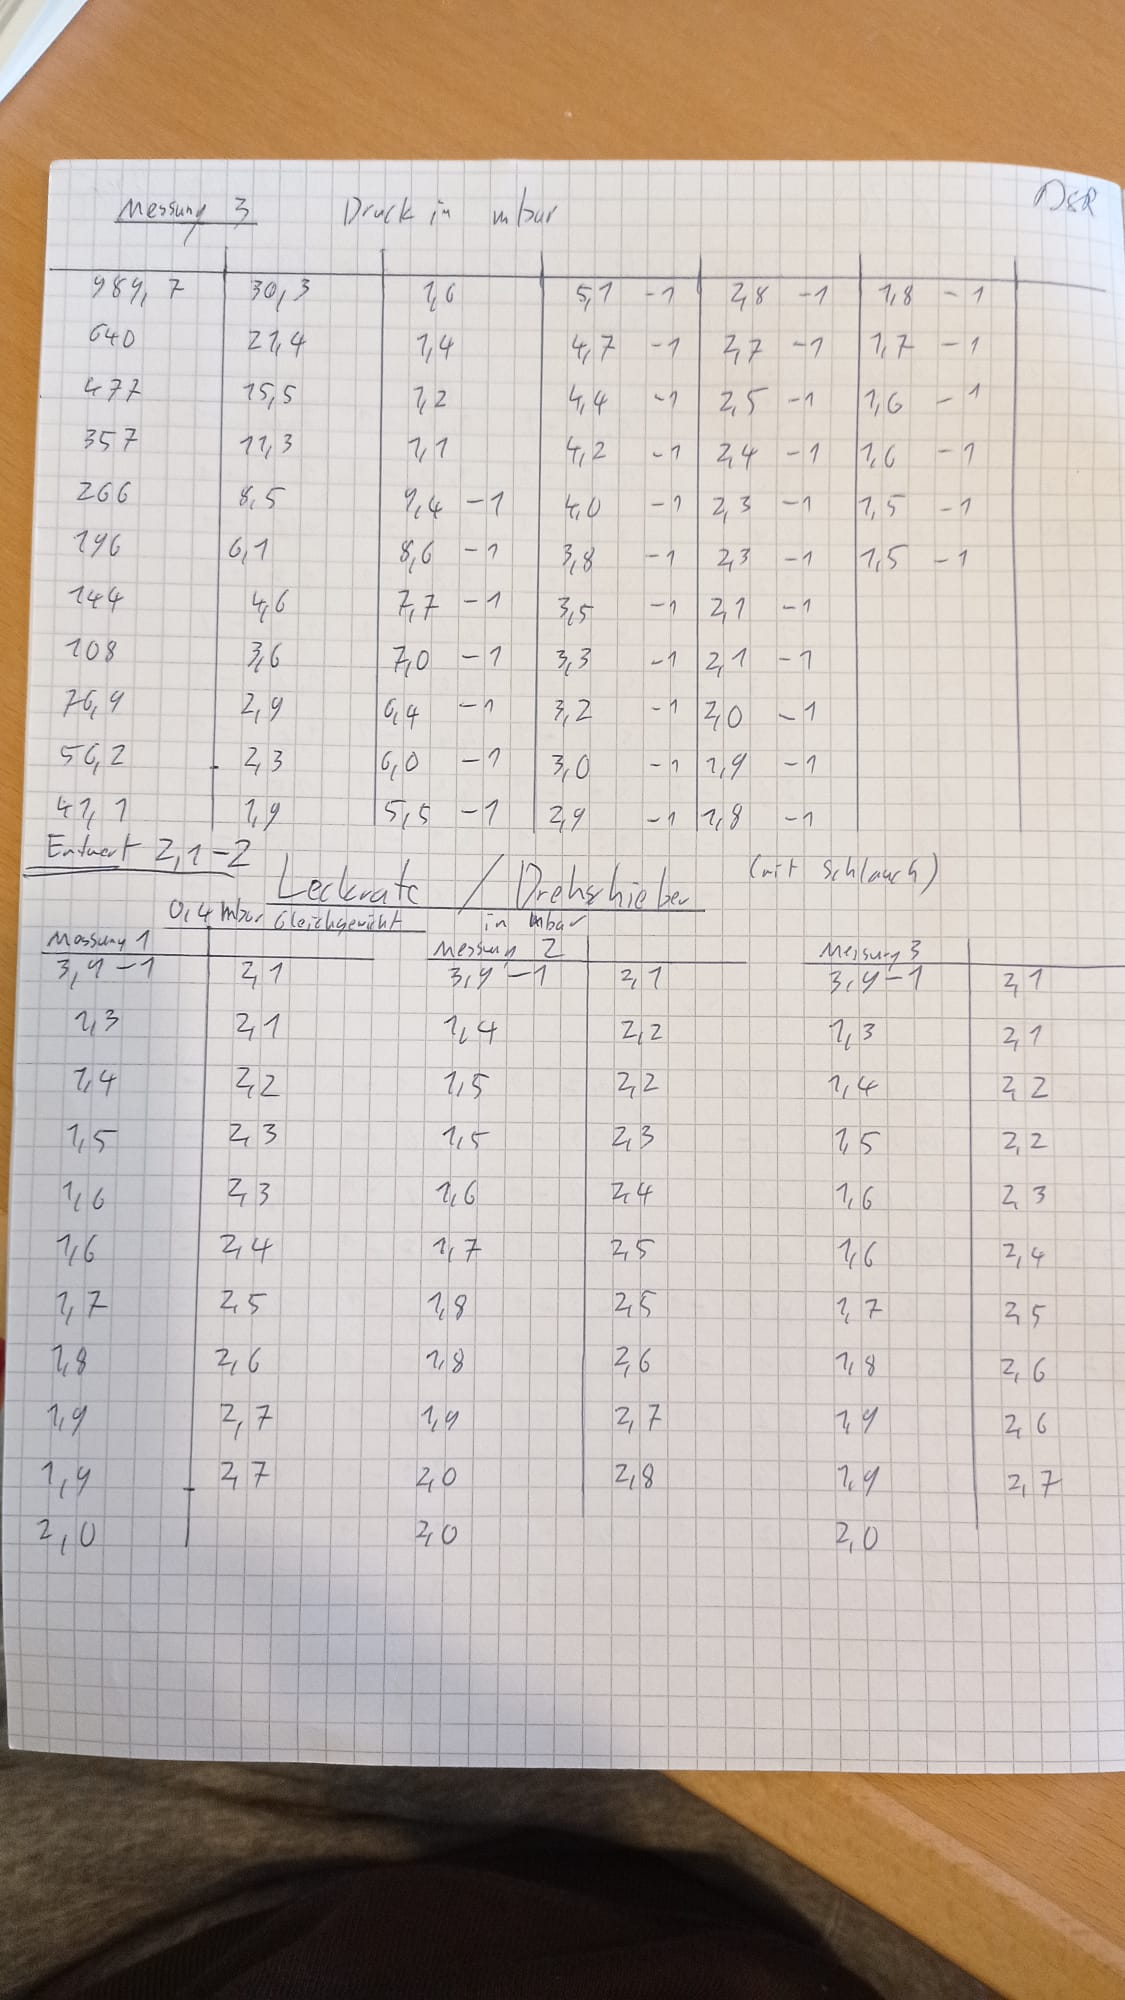
\includegraphics[width=0.7\textwidth]{latex/images/Messwerte_6.jpeg}
    \caption{Die Messwerte des Vakuumversuchs}
\end{figure}


\begin{figure}[h]
    \centering
    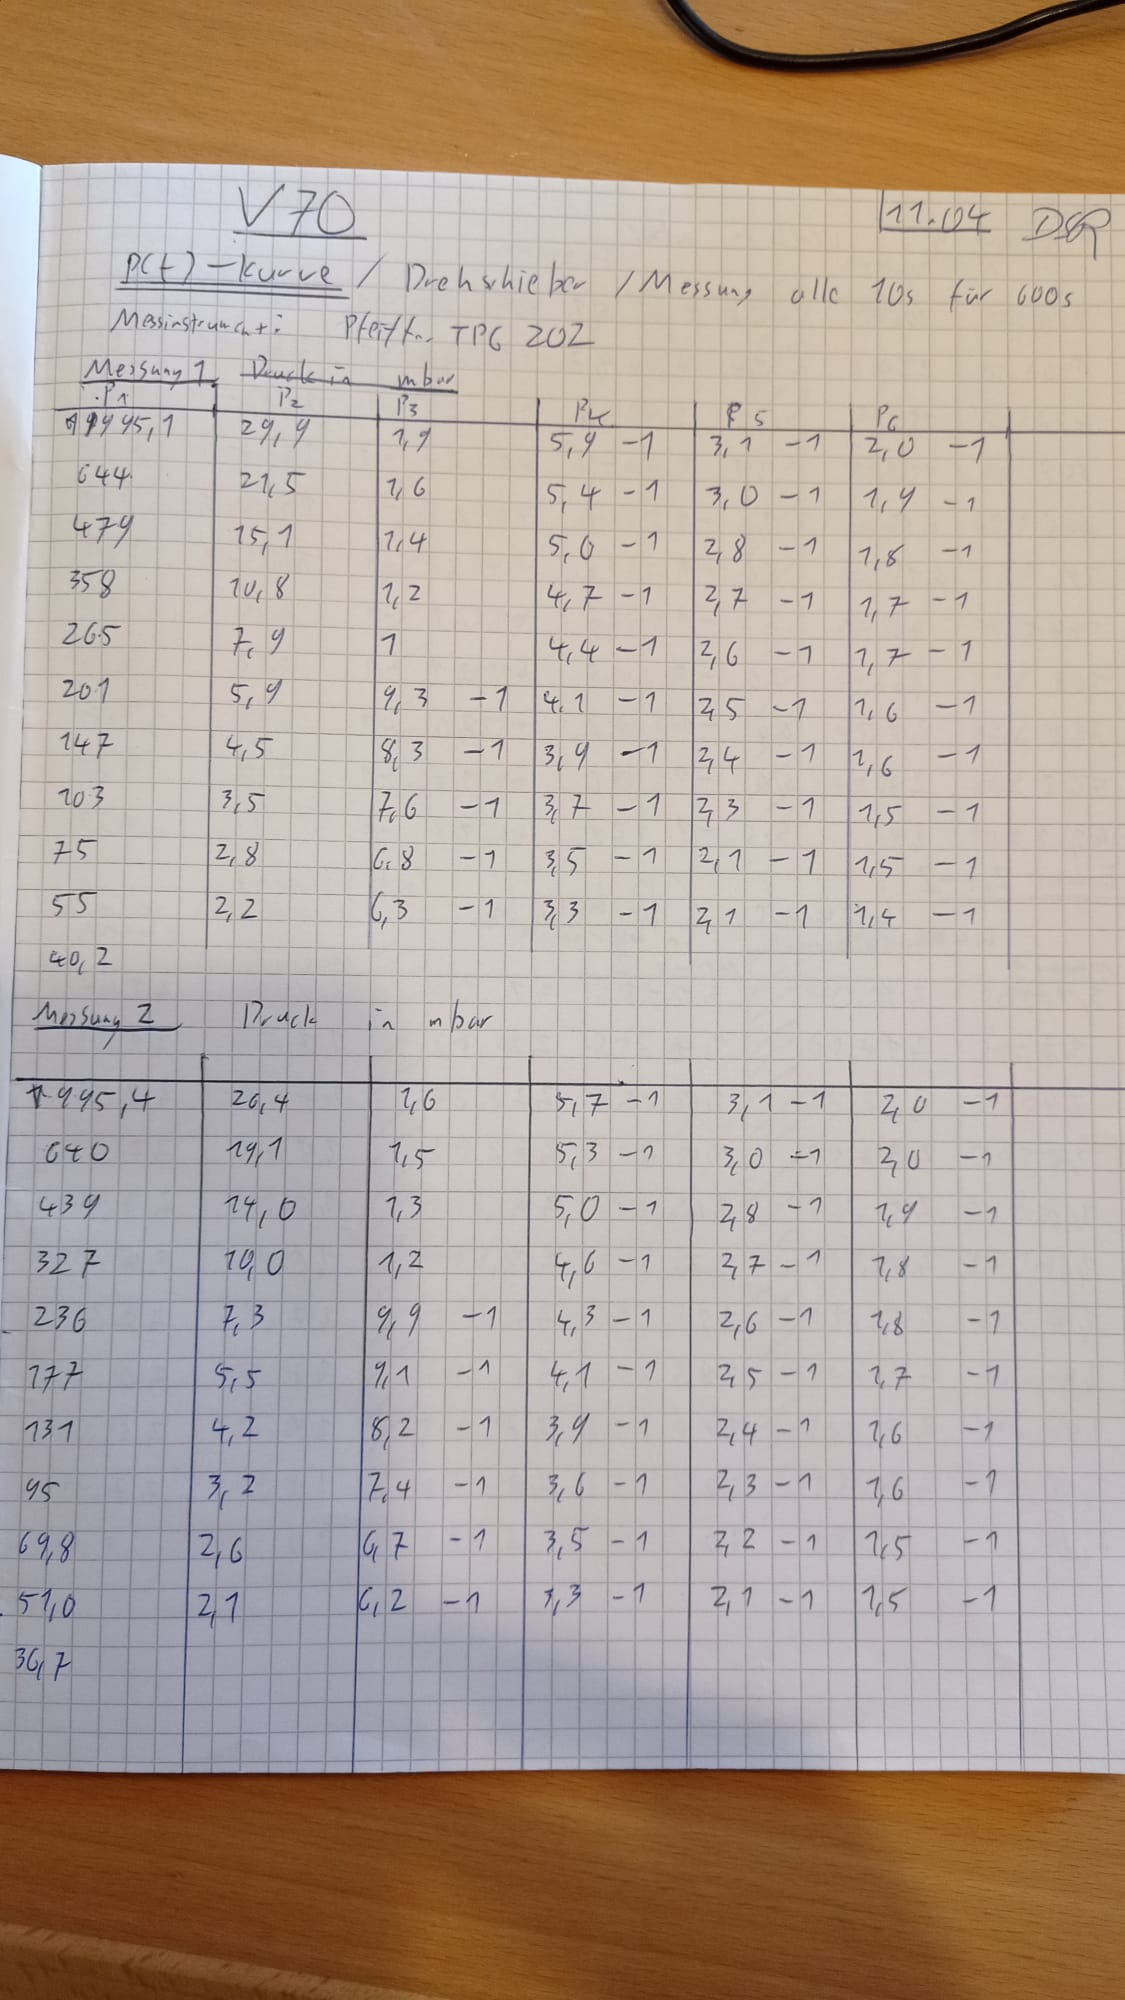
\includegraphics[width=0.7\textwidth]{latex/images/Messwerte_7.jpeg}
    \caption{Die Messwerte des Vakuumversuchs}
\end{figure}

\begin{figure}[h]
    \centering
    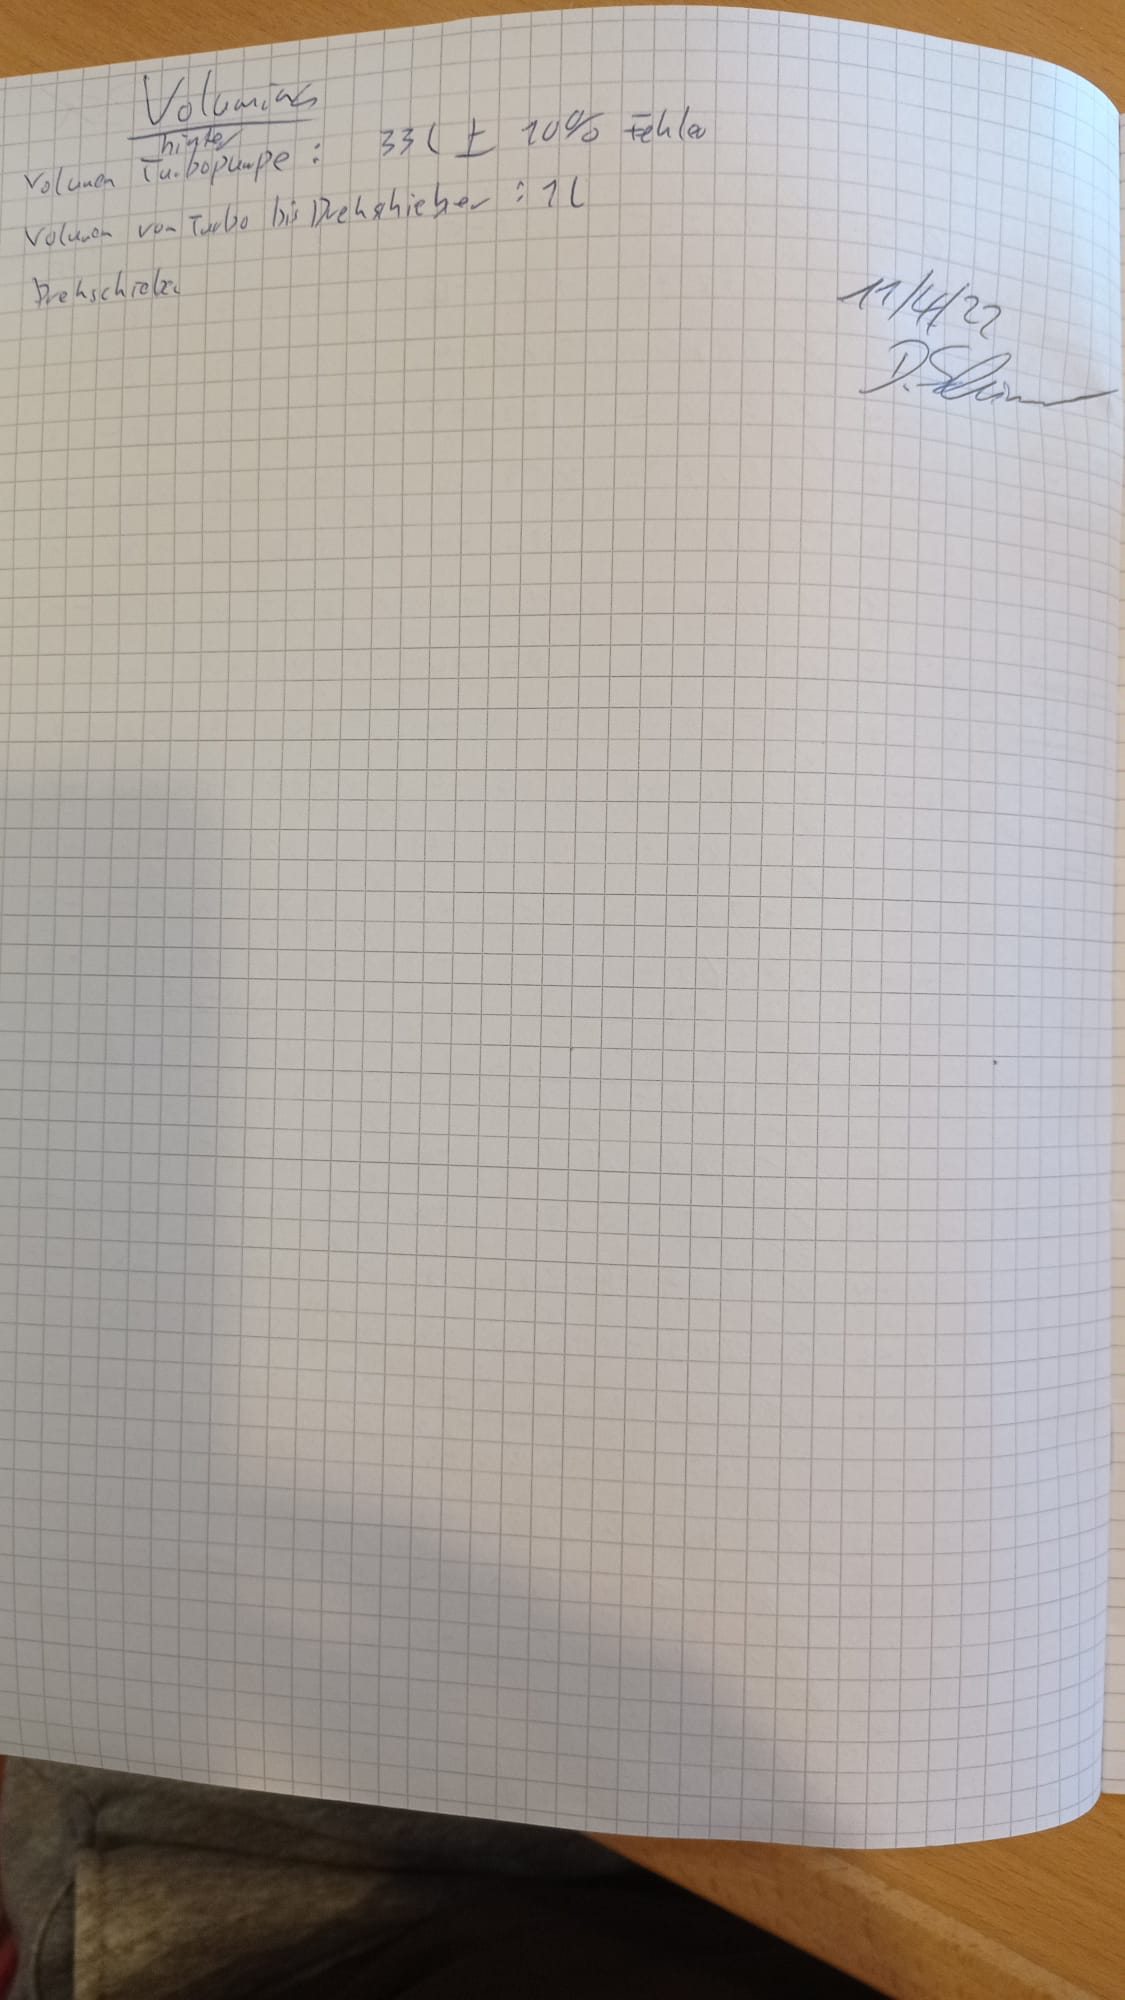
\includegraphics[width=0.7\textwidth]{latex/images/Messwerte_8.jpeg}
    \caption{Die Messwerte des Vakuumversuchs}
\end{figure}



